\chapter{Ermittlung der Funkreichweite}
\label{ch:Reichweite}
Die Ermittelung der Reichweite dient dazu, das nötige Sendeintervall zu bestimmen.
Die Reichweite wurde bisher als 50 Meter angenommen, das Sendeintervall dementsprechend auf 5 Sekunden gesetzt.
In dieser Zeit kann ein Mitarbeiter maximal 42 Meter bei einer Geschwindigkeit von 30 km/h bewegen. 
Für den anschließenden Vergleich sollen jedoch realistische Bedingungen, mit einem für die Funkcharakteristik des Tunnels angepassten Sendeintervall, geschaffen werden.

\section{WLAN}
Für die Tests wurde ein LN-862 Access Point von der Firma Lancom zur Verfügung gestellt.
Dieser wurde am hinteren Ende einer Tunnelbohrmaschine montiert.\\
Die Tunnelbohrmaschine befindet sich in der Tunnelbaustelle Rastatt. 
Der Durchmesser des Bahntunnels beträgt 9 Meter, das Ende der Tunnelbohrmaschine befand zum Zeitpunkt der Messungen circa 2 Kilometer weit im Tunnel.\\
Der AP konnte aufgrund des geringen Platzangebots und den wenigen zur Verfügung stehenden Steckdosen nicht frei platziert werden.
Er wurde deshalb unter der ersten stählernen Treppe platziert, diese beeinträchtigt natürlich das Signal.
Da es aber üblich ist IT-Gerätschaften, wie die derzeit verwendeten Bluetooth-Basisstationen, in Metallboxen zu verstauen um sie vor äußeren Einflüssen zu schützen, ist eine gewisse Abschirmung durchaus realitätsnah.
Die Platzierung des AP ist auf Abbildung \ref{fig:tunnelmark} eingezeichnet.\\
Abbildung \ref{fig:applacement} zeigt den LN-862 hinter der Treppe.

\begin{figure}[h]
  \centering
	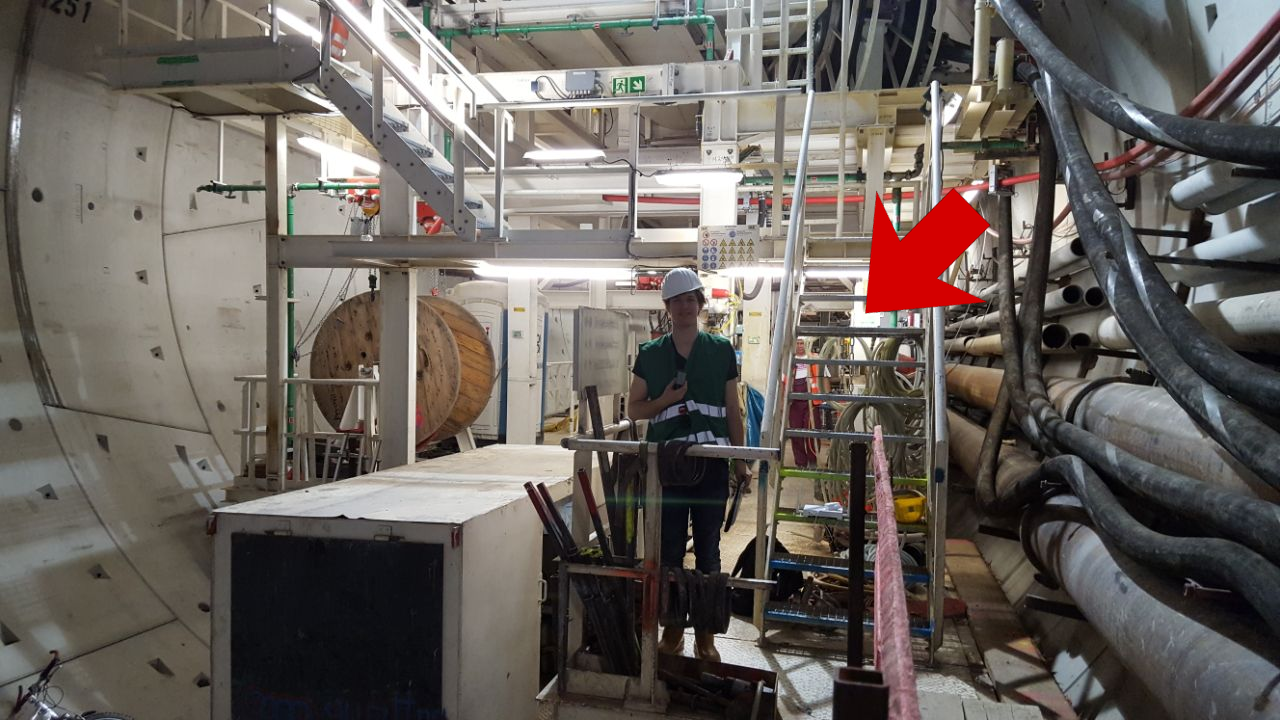
\includegraphics[width=\textwidth]{images/tunnelmark.png}
  \caption{Ende der Tunnelbohrmaschine, Pfeil markiert Platzierung des Access Point hinter der Treppe.}
  \label{fig:tunnelmark}
\end{figure}

\begin{figure}[h]
  \centering
	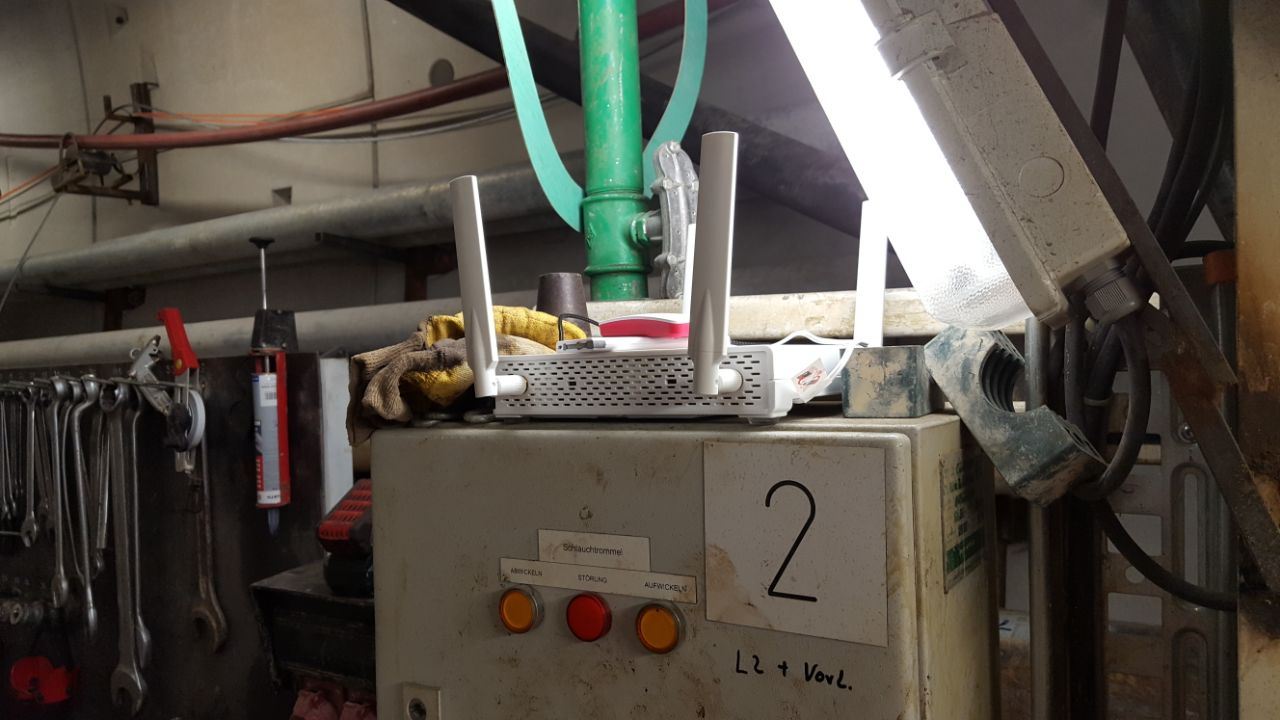
\includegraphics[width=\textwidth]{images/applacement.jpg}
  \caption{LN-862 im Tunnel, darauf liegt der Pi Zero W.}
  \label{fig:applacement}
\end{figure}

\subsection{Methodik}
Die Reichweite in zwei Richtungen geprüft.
Zum einen in Richtung des bereits fertig gebohrten Tunnels, hier blockiert nur wenig Stahl das Signal. 
Lediglich die Treppe, unter der der AP montiert wurde, stellt ein Hindernis dar.
Zum anderen wurde die Reichweite in Richtung des Vortriebs geprüft.
Dabei stellen eine stählerne Zwischendecke und große Container Hindernisse dar.\\
Außerdem wird die Abschrimung durch ein Gehäuse getestet.
Dazu wurde eine stabile Plastikbox verwendet, leider konnte diese für den Versuch mit der Bleutooth-basierten mobilen Einheit nicht vollends geschlossen werden.\\
Für die Messung wurde der Körper zwischen mobiler Einheit und Basisstation gebracht und eine mobile Einheit wurde dann als "außer Reichweite" angesehen, wenn versendete Pakete der mobilen Einheit nicht mehr bei der Basisstation ankamen.
In jedem Fall war es möglich durch das Entfernen des körperlichen Hindernisses wieder eine Verbindung herzustellen.\\
Zur Bestimmung der Distanz wurden die Tübbinge verwendet, dies sind Schalungselemente im Tunnel.
Im Tunnel Raststatt sind diese fortlaufend nummeriert und genau zwei Meter breit, die Messungen sind deshalb ebenfalls in zwei Meter Schritten angegeben.

\subsection{Ergebnisse}
Tabelle \ref{table:rangewifi} zeigt die Ergebnisse für die zwei verwendeten ESP8266 Module.
Es wurde jeweils mit und ohne Gehäuse gemessen und in jede der beiden beschriebenen Richtungen.
Wenige Hindernisse bezeichnet dabei die Richtung des bereits fertig gebohrten Tunnels, viele Hindernisse die Richtung des Vortriebs.

\begin{table}[h]
	\centering
	\caption{Sendereichweite WLAN-basierter mobiler Einheiten}
	\label{table:rangewifi}
	\begin{tabular}{p{3.5cm}|p{3cm}|p{3.5cm}|p{3cm}}
		Verwendetes Modul & Aufbau & Strecke & Maximale Sendereichweite \\
		\hline
		ESP-12E & Offen & Wenige Hindernisse & 84m \\
		ESP-12E & In Gehäuse & Wenige Hindernisse & 74m \\
		ESP-12E & Offen & Viele Hindernisse & 26m \\
		ESP-12E & In Gehäuse & Viele Hindernisse & 30m \\
		\hline
		ESP-12F & Offen & Wenige Hindernisse & 88m \\
		ESP-12F & In Gehäuse & Wenige Hindernisse & 88m \\
		ESP-12F & Offen & Viele Hindernisse & 32m \\
		ESP-12F & In Gehäuse & Viele Hindernisse & 32m \\
	\end{tabular}
\end{table}


\subsection{Bewertung}
\label{ch:Reichweite:sec:bewertung}
Das ESP-12F Modul hatte in jedem der vier Testszenarien eine höhere Reichweite als das ESP-12E, es ist daher im weiteren Verlauf zu bevorzugen.\\
Die bisher angenommenen 50 Meter Reichweite sind für dieses Modul deutlich zu vorsichtig geschätzt. 
Um die gemessenen 88 Meter bei 30 km/h zu durchqueren benötigte ein Mitarbeiter circa 10,5 Sekunden, bei einem Sendeintervall von zehn Sekunden finden demnach zwei Sendevorgänge beim durchqueren des Einflussbereichs eines APs statt.
Da eine zuverlässige Erkennung von Bereichswechseln gefordert wurde, sollte das Sendeintervall konservativer auf acht Sekunden gesetzt werden.\\
Für die Teststrecke mit vielen Hindernissen wurden geringere Reichweiten gemessen, eine solche Teststecke findet sich aber nur auf der Tunnelbohrmaschine, welche nur zu Fuß begangen werden kann. 
Geht man von einer maximalen Bewegungsgeschwindigkeit von zehn km/h für eine laufende Person aus durquerte diese in acht Sekunden 22 Meter, also deutlich weniger als die gemessenen 32 Meter.\\





\section{Bluetooth}
Der Versuch mit Bluetooth wurde an der selben Stelle wie der mit WLAN durchgeführt.
Es wurde allerdings ein Raspberry Pi Zero W als Basisstation verwendet, dieser wurde auf dem LN-862 platziert, auf Abbildung \ref{fig:applacement} ist sein rotes Gehäuse zu erkennen.

\subsection{Methodik}
Die Reichweite wurde erneut in zwei Richtungen geprüft. 
Zum einen in Richtung der fertig gebohrten Tunnels mit wenigen Hindernissen, zum anderen in Richtung des Vortriebs durch mehrere Stahlhindernisse.
Um die Abschirmung durch ein Gehäuse zu simulieren wurde eine stabile Plastikbox verwendet, leider konnte diese nicht vollends geschlossen werden.\\
Für die Messung wurde der Körper zwischen mobile Einheit und Basisstation gebracht und eine mobile Einheit wurde dann als "außer Reichweite" angesehen, wenn versendete Pakete der mobilen Einheit nicht mehr bei der Basisstation ankamen.
Durch das Entfernen des körperlichen Hindernisses war es möglich wieder eine Verbindung herzustellen.\\
Die bestimmten Reichweiten werden in zwei Meter Schritten angegeben, da sie mit Hilfe der zwei Meter breiten Tübbing Elemente bestimmt wurden.

\subsection{Ergebnisse}
Tabelle \ref{table:rangeblue} zeigt die Ergebnisse für den nRF52.
Für diesen sind keine Ergebnisse mit geschlossenem Gehäuse aufgeführt, denn das Gehäuse ließ sich für diesen Prototyp nicht schließen.
Das lose Auflegen des Deckels führte zu keiner Veränderung bei der Reichweite.

\begin{table}[h]
	\centering
	\caption{Sendereichweite Bluetooth-basierter mobiler Einheiten}
	\label{table:rangeblue}
	\begin{tabular}{p{3.5cm}|p{3cm}|p{3.5cm}|p{3cm}}
		Verwendetes Modul & Aufbau & Strecke & Maximale Sendereichweite \\
		\hline
		nRF52 & Offen & Wenige Hindernisse & 32m \\
		nRF52 & Offen & Viele Hindernisse & 14m \\
	\end{tabular}
\end{table}

\subsection{Bewertung}
Auch die mobile Einheit auf Bluetooth Basis hat eine höhere Reichweite als zunächst angenommen. 
Dennoch lohnt sich eine Anpassung des Sendeintervalls für die Lösung nicht, da der Großteil des Verbrauchs der mobilen Einheit passiv über die angrenzenden Komponenten wie Spannungswandler und Lithium-Akku-Ladeschaltkreis erfolgt.





\section{LoRa}
Die Versuche mit LoRa wurden an einer anderen Tunnelbaustelle durchgeführt.
An der Tunnelbohrstelle Ulm wird mit Sprengungen vorgetrieben.
Nach der Sprengung wird der Tunnel mit Spritzbeton ausgekleidet und danach wird in drei Schritten geschalt. 
Im ersten Schritt wird ein Filz und eine Folie gegen das Eindringen von Wasser eingebracht, danach folgt die Bewehrung und abschließend wird die Bewehrung einbetoniert.
Für jeden Schritt wird ein stählerner Schalungswagen verwendet, folglich sind drei stählerne Hindernisse im Tunnel, die Signale absorbieren.
Abbildung \ref{fig:schalungswagen} zeigt einen der Schalungswagen, der als Hindernis gedient hat.

\begin{figure}[h]
  \centering
	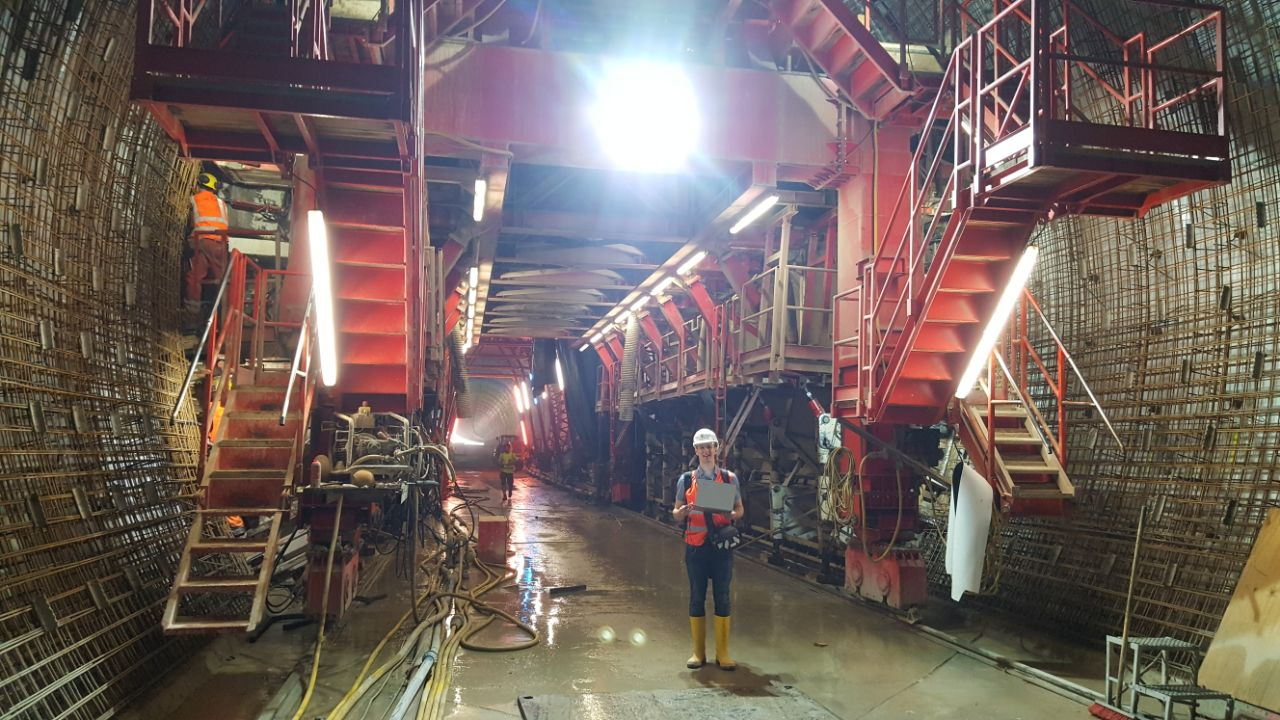
\includegraphics[width=\textwidth]{images/schalungswagen.jpg}
  \caption{Schalungswagen für daa Betonieren im Tunnel Ulm.}
  \label{fig:schalungswagen}
\end{figure}

\subsection{Methodik} 
Die Reichweite wurde für 2 Situationen bestimmt.
Zum einen durch einen Schalungswagen und dann durch den freien Tunnel, zum anderen durch alle drei Schalungswagen für eine Situation mit maximaler Abschirmung durch die Hindernisse.
Die mobile Einheit wurde jeweils direkt an der Bewehrung platziert und es wurde auf der selben Seite gelaufen, damit die Abschirmung durch die Schalungswagen maximal ist.
Danach wurde die Basisstation immer weiter entfernt, bis keine Pakete der mobilen Einheit mehr empfangen werden konnten.
Abbildung \ref{fig:lorabasis} zeigt die Platzierung der mobilen Einheit an der Bewehrung.
Erneut konnte die Plastikbox aufgrund des Versuchsaufbaus nicht geschlossen werden.
Die mobile Einheit wurde als "außer Reichweite" angesehen, wenn versendete Pakete der mobilen Einheit nicht mehr bei der Basisstation ankamen.
Durch das Entfernen des körperlichen Hindernisses war es möglich wieder eine Verbindung herzustellen.
Es wurde sowohl mit einer Sendeleistung von 5dBm für einen geringen Sendeverbrauch als auch mit 23dBm Sendeleistung für maximale Reichweite gemessen.
Die Messungen werden in 12,5 Meter Abständen angegeben, da in diesem Tunnel die Länge eines Schalungselements 12,5 Meter beträgt.
Es werden, wie in Abschnitt \ref{ch:hardwarechanges:sec:rfm95} besprochen zwei unterscheidliche Typen von Antennen verwendet. 
Während die Basisstation eine feste Antenne aufweist, verwendet die mobile Einheit eine Kabelantenne entsprechend der halben Wellenlänge. 

\begin{figure}[h]
  \centering
	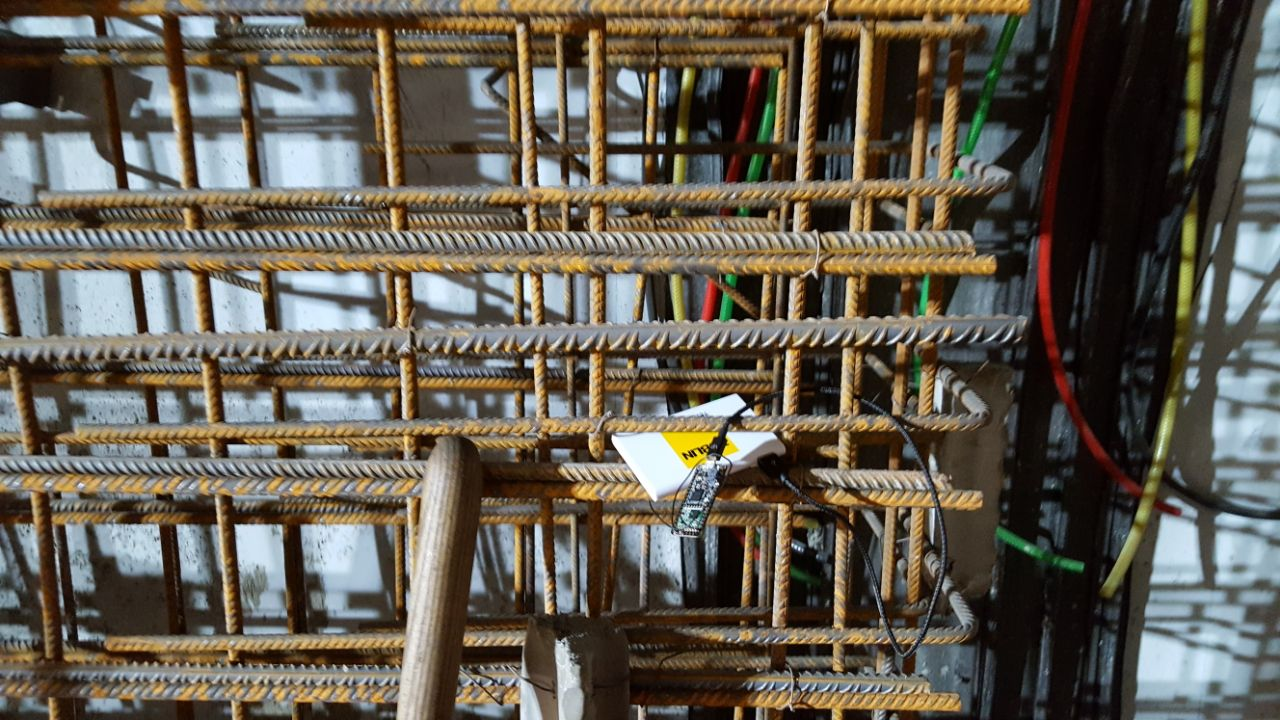
\includegraphics[width=\textwidth]{images/lorabasis.jpg}
  \caption{Platzierung der mobilen Eiheit an der Bewehrung des Tunnels.}
  \label{fig:lorabasis}
\end{figure}

\subsection{Ergebnisse}
Tabelle \ref{table:rangelora} zeigt die Ergebnisse für das RFM95.
Da das lose Auflegen des Deckels der Plastikbox zu keiner Veränderung bei der Reichweite führte gibt die Tabelle nur Werte für den offenen Aufbau an. 
Der Test mit 23dBm Sendeleistung durch alle drei Schalungswagen musste nach 350 Metern abgebrochen werden, weil ein weiterkommen nicht möglich war.
Da jedoch für diese Sendeleistung bereits nach circa 250 Metern die Varianz des RSSI den Zusammenhang zwischen Distanz und RSSI überwiegt, kann die tatsächliche Reichweite dieser Sendeleistung nicht ausgenutzt werden.
Für eine sichere Erkennung des 250-Meter-Abschnitts müsste daher alle 500 Meter eine Basisstation aufgestellt werden.

\begin{table}[h]
	\centering
	\caption{Sendereichweite LoRa-basierter mobiler Einheiten}
	\label{table:rangelora}
	\begin{tabular}{p{2.2cm}|p{1.5cm}|p{2.5cm}|p{3.5cm}|p{3cm}}
		Verwendetes Modul & Aufbau & Sendeleistung & Strecke & Maximale Sendereichweite \\
		\hline
		RFM95 & Offen & 5dBm & Wenige Hindernisse & 250m \\
		RFM95 & Offen & 5dBm & Viele Hindernisse & 100m \\
		\hline
		RFM95 & Offen & 23dBm & Wenige Hindernisse & 1250m \\
		RFM95 & Offen & 23dBm & Viele Hindernisse & >350m \\
	\end{tabular}
\end{table}

\subsection{Bewertung}
LoRa entfaltet im Tunnel eine sehr hohe Reichweite und es kann eine lückenlose Überwachung von Personen durchgeführt werden.
Voll nutzen lässt sich diese jedoch nicht, da die Varianz des RSSI den Zusammenhang zwischen Distanz und RSSI schon nach circa 250 Metern überwiegt. 
Hingegen führt eine starke Reduktion der Sendeleistung zu einer mangelden Penetration von Hindernissen.
Daher sollte ein Kompromiss der Sendeleistung geschlossen werden. 
Eine Sendeleistung von 10dBm sollte eine ausreichende Reichweite im Szenario mit vielen Hindernissen bieten.
Alternativ kann die mobile Einheit auch ein Send-Receive Schema umsetzen und von der Basisstation eine dynamisch angepasste Sendeleistung empfangen, die sich nach der Menge der Hindernisse richtet.


